% 20200713
\documentclass[../thesis.tex]{subfiles} %% use packages & commands as this main file
\begin{document}
\section{Methodology}

\subsection{The model}

This system contained two biological components (i.e. phytoplankton and bacteria) and three state variables of densities (i.e. organic carbon $C$, phytoplankton biomass $P$ and bacterial biomass $B$) under a standardised temperature range of \temp.  Both biological components received carbon from different sources but performed the same functions. Phytoplankton photosynthesized carbon dioxide from the atmosphere (an unlimited source) while bacteria consumed organic carbon from its environment.  Both phytoplankton and bacteria respired and leaked a fraction of the carbon obtained respectively and allocated the rest to its biomass; some of the biomass died and became organic carbon in the environment.  Organic carbon in the environment could either be consumed by the bacteria or harvested from the system.  In this study we had four major assumptions: 1. living conditions in the system was homogeneous spatially, nutritionally, carbon and light availability; 2. unlimited nutrient supply from the utilization of sewage \autocite{markou2014microalgal}; 3. high carbon density would not block light for phytoplankton; and 4. bacteria do not have preference on the type of carbon as its resource.  In short, this model had only one explicit environmental limitation -- living space for phytoplankton.

Equations were listed as the rate of density change of state variables (grams of carbon per metre cube per day, \dxdt).  Three state variables of densities, two sets of four biological parameters (one set for $P$ and another set for $B$) and one harvest rate parameter was included in this minimal carbon cycle model.

\begin{equation}\left\{\begin{array}{rl}
    C'(t) &= \ePR(1-\eP)\cdot\gP\cdot P +\aP\cdot P^2 +(\eBR(1-\eB)-1)\cdot\gB\cdot C\cdot B +\mB\cdot B -xC\\
    P'(t) &= \ePR\cdot\eP\cdot\gP\cdot P -\aP\cdot P^2\\
    B'(t) &= \eBR\cdot\eB\cdot\gB\cdot C\cdot B -\mB\cdot B
\end{array}\right.\label{eq:PBH}\end{equation}

In Eq.\ref{eq:PBH}, $C'(t)$, $P'(t)$ and $B'(t)$ were the rate of change of densities (unit \dxdt).  $\ePR$ was the fraction of non-respired carbon for $P$, $\eP$ was the fraction of carbon incorporated as $P$ biomass, $\eBR$ was the fraction of non-respired carbon for $B$ and $\eB$ was the fraction of carbon incorporated as $B$ biomass.  The above four unitless parameters were grouped as “fraction parameters”.  $\gP$ was the growth rate of $P$ (\dayU), $\aP$ was the intraspecific interference of $P$ (\denI), $\gB$ was the resource clearance rate of $B$  (\denI) and $\mB$ was the death rate of $B$ (\dayU).  These four were the “rate parameters”.  $x$ was the harvest rate (\dayU) which determined how fast the carbon in the environment got removed.  Below was the graphical version of our model.

\begin{figure}[H]
    \centering
    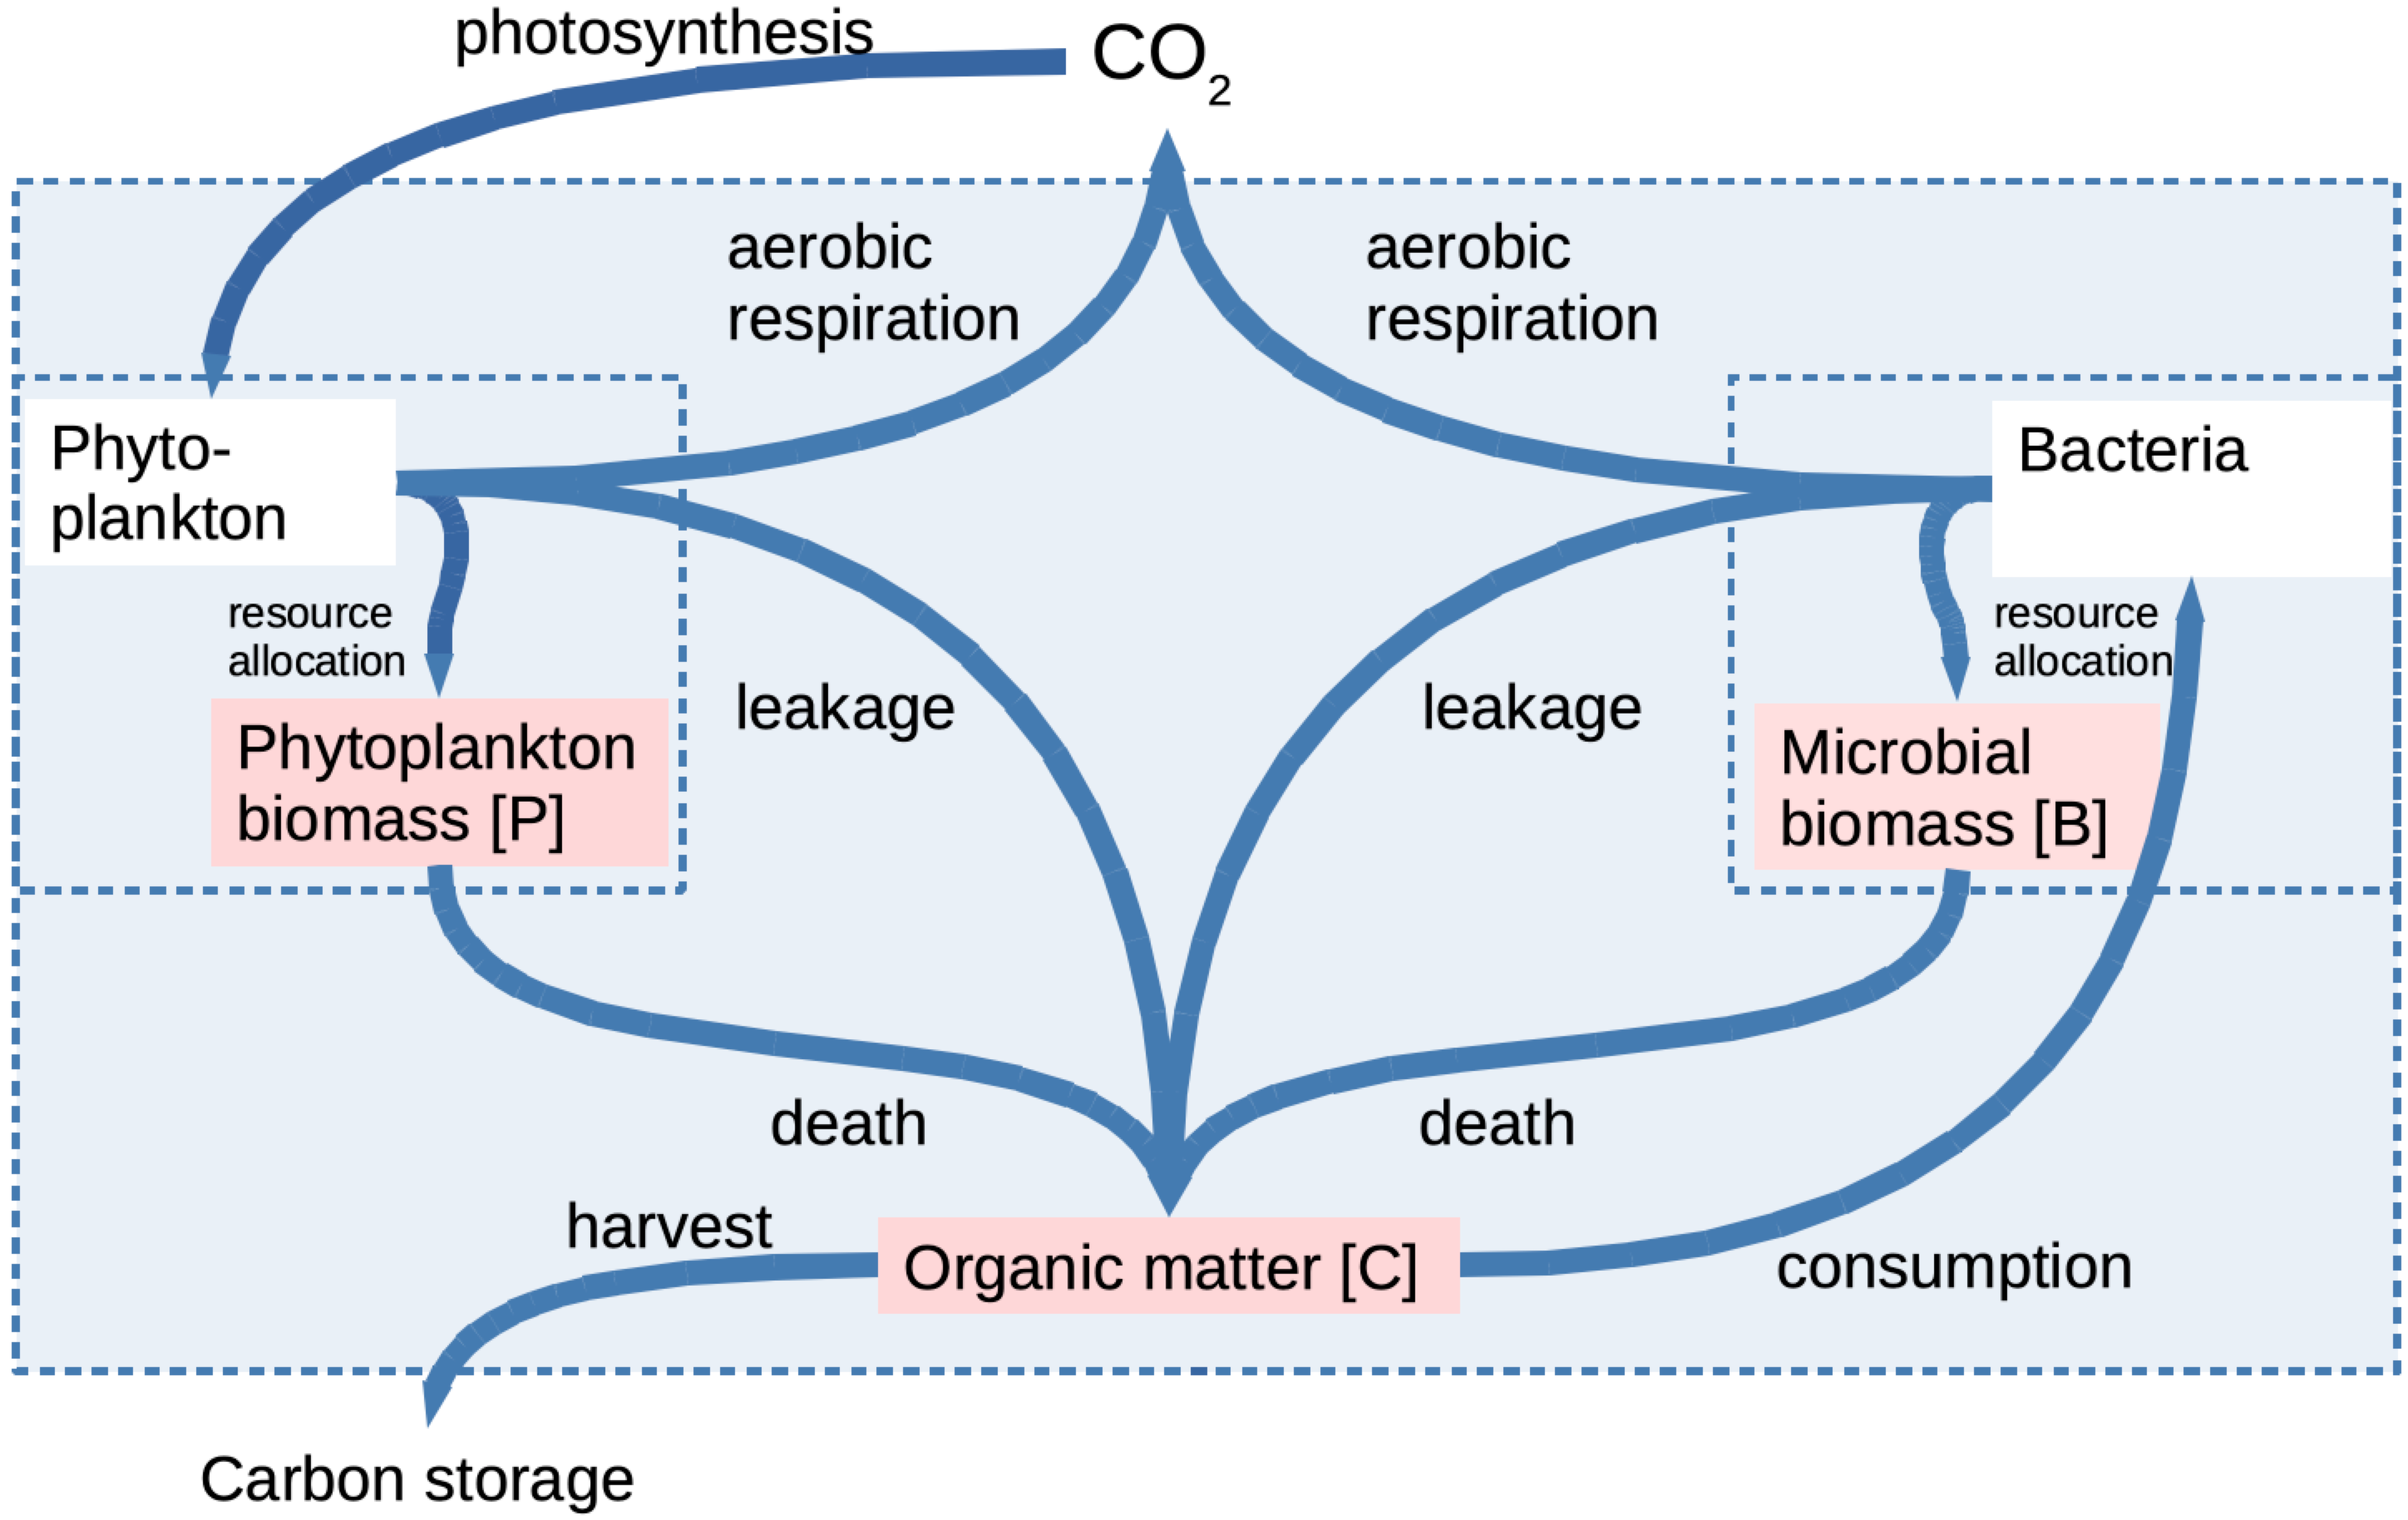
\includegraphics[width=.8\linewidth]{media/model.png}
    \caption[Model visualization]{The theoretical coexistence open system of phytoplankton and bacteria.  Dashed boxes were the defined boundaries, which the large box defined the open system for matter exchange, the box contained phytoplankton resembles the cellular boundaries of phytoplankton and the box contained bacteria resembles the cellular boundaries of bacteria.  Blue arrows indicated the direction of carbon densities flow from a resource pool to another.  Text above the arrows were the biological processes represented by the arrows.  Pink boxes represented the carbon density pools defined by the state variables, which were the states of which the carbon in the system could be identified.  White boxes represented the functional components of the biological components in the system.  Biologically the white boxes were the collection of all biochemical reactions within the whole population of organisms indicated in the text of respective boxes.}
    \label{f:model}
\end{figure}

Eq.\ref{eq:PBH} was simulating the setting of $B$ coexisting with $P$ under continuous harvest (\PBH).  The full-geared model had three other alternative forms:

P-only with harvest (\PoH);
\begin{equation}\left\{\begin{array}{rl}
    C'(t) &= \ePR(1-\eP)\cdot\gP\cdot P +\aP\cdot P^2 -xC\\
    P'(t) &= \ePR\cdot\eP\cdot\gP\cdot P -\aP\cdot P^2
\end{array}\right.\label{eq:PoH}\end{equation}

$B$ coexist with $P$ without continuous harvest (\PBN); and
\begin{equation}\left\{\begin{array}{rl}
    C'(t) &= \ePR(1-\eP)\cdot\gP\cdot P +\aP\cdot P^2 +(\eBR(1-\eB)-1)\cdot\gB\cdot C\cdot B +\mB\cdot B\\
    P'(t) &= \ePR\cdot\eP\cdot\gP\cdot P -\aP\cdot P^2\\
    B'(t) &= \eBR\cdot\eB\cdot\gB\cdot C\cdot B -\mB\cdot B
\end{array}\right.\label{eq:PBN}\end{equation}

P-only without continuous harvest (\PoN).
\begin{equation}\left\{\begin{array}{rl}
    C'(t) &= \ePR(1-\eP)\cdot\gP\cdot P +\aP\cdot P^2\\
    P'(t) &= \ePR\cdot\eP\cdot\gP\cdot P -\aP\cdot P^2
\end{array}\right.\label{eq:PoN}\end{equation}

Upon rearranging the variables in the above four system alternatives by SymPy (v1.5.1) in python3 (v3.7.3), we got six possible stable system states.

\begin{table}[H]
    \centering
    \caption{Table of equilibria from the four variations of the proposed model (Eq.\ref{eq:PBH})}
    \begin{tabular}{cl|ccc}\hline
        equilibrium & scenario & $C$ & $P$ & $B$ (only if scenario contained $B$) \\\hline
        1 & \PBH, \PoH & 0 & 0 & 0 \\
        2 & \PBH & $\dfrac{\mB}{\eBR\eB\gB}$ & 0 & $\dfrac{-x}{\gB(1-\eBR)}$ \\
        3 & \PBH, \PoH & $\dfrac{\eP(\ePR\gP)^2}{\aP x}$ & $\dfrac{\ePR\eP\gP}{\aP}$ & 0 \\
        4 & \PBH & $\dfrac{\mB}{\eBR\eB\gB}$ & $\dfrac{\ePR\eP\gP}{\aP}$ & $\dfrac{(\ePR\gP)^2\eBR\eB\gB-\aP\mB x}{(1-\eBR)\aP\gB\mB}$ \\
        5 & \PBN & C & 0 & 0 \\
        6 & \PoN & - & P & - \\\hline
    \end{tabular}
    \label{t:eqm}
\end{table}

Among all the possible states, only defined positive states were biologically possible because densities cannot be negative.  Equilibrium 5 and 6 were not defined; equilibrium 1 contained no biological meaning and equilibrium 2 was not biologically possible.  Hence we only had equilibrium 3 and 4 left, which resembled the setting of \PoH\ and \PBH respectively.

\subsection{Parameter space}
Not all defined parameters in our model had experimentally measured values.  Also, there was not a single species with published measurements on every biological parameter we defined.  Luckily there was at least one available value for each biological parameter in our model.  Hence in this study, we used a percentage range of known parameters to narrow down the unknown ranges of biological parameters with limited data and uniform prior to set sampling points within the parameter ranges of each biological parameters.  Ranges of each biological parameter was listed below and details of how we determined each biological parameter range was in the appendix.

\begin{table}[H]
    \centering
    \caption[Algebra variables]{Table showing biological variables and corresponding ranges framing the parameter space}
    \begin{tabular}{cclll}\hline
        variable & unit & description & min & max \\\hline
        $N'(t)$ & \dxdt & rate of change of respective carbon pool {\tiny($N=C,P,B$)} & - & - \\
        $N$ & \den & carbon density for respective pool {\tiny($N=C,P,B$)} & - & - \\
        $\ePR$ & - & non-respired carbon fraction for $P$ & 0.08 & 0.87 \\
        $\eP$ & - & assimilated carbon fraction for $P$ & 0.40 & 1.00 \\
        $\gP$ & \dayU & growth rate of $P$ & 0.03 & 3.17 \\
        $\aP$ & \denI & intraspecific interference of $P$ & 0.02 & 1.52 \\
        $\eBR$ & - & non-respired carbon fraction for $B$ & 0.13 & 1.00 \\
        $\eB$ & - & assimilated carbon fraction for $B$ & 0.07 & 0.82 \\
        $\gB$ & \denI & clearance rate of $B$ & 0.10 & 3.50 \\
        $\mB$ & \dayU & death rate of $B$ & 0.01 & 0.63 \\
    \hline\end{tabular}
    \label{t:ranges}
\end{table}

\subsection{Scenario sampling}
Within the parameter ranges using the uniform prior, we selected 11 values in the regular interval for each parameter using R (v4.0.2).  Next we randomly arranged the values for each parameter so that each parameter combination was unique.  This step was called a Latin Hypercube Sampling (LHS).  To ensure the study’s reproducibility, we had set the seed for random numbers to ``20192020”.  Then we expanded the LHS to 500 unique sets of parameter combinations and applied 200 harvest rates (for continuous harvest systems) or intervals (for destructive harvest systems) of regular interval ranged from 1 to 19901 \dayU.  The total number of scenarios was hence 1.1 million ($11\times500\times200$).

\subsection{Model experiment}
C (compiler gcc v7.5.0) was used for analytical calculations on continuous harvest systems (equilibrium 3\&4 in Table \ref{t:eqm}).  Yield flux was defined by $x\cdot C$ in Eq.\ref{eq:PBH}, and hence the calculation showed \PoH\ systems were independent of harvest rate (Table \ref{t:eqm}).

Python3 SciPy (v1.2.3) package ``odeint" function was chosen for numerical integrations on the destructive harvest systems (Eq.\ref{eq:PBN}\&\ref{eq:PoN}).  We used Eq.\ref{eq:PBH} by tweaking harvest rate parameter and initial densities because destructive harvest systems were variations from \ref{eq:PBH}.  Hence by setting $x=0$, we ran \PBN\ systems by initial densities of $C=P=B=1$ \den\ and \PoN\ systems by $C=P=1$ and $B=0$ \den.  We defined the daily yield flux as the average yield difference in each ``wait and replace" cycle.  Hence it was calculated as $\dfrac{[\text{total carbon on harvest day}]-[\text{total carbon on initial day}]}{[\text{day passed}]}$ with initial day equal to day 1.

\subsection{Analysis of carbon density yield fluxes}
We performed pairwise Wilcox signed rank tests on all necessary occasions (in R) with bonferroni p-value adjustment and no paired situations to check on their difference in medians.  Since harvest rates and harvest intervals were the same in units but different in logic, we selected three harvest values differed in magnitude (101, 1001, 10001) to compare the two harvest systems (\PBH\ vs \PoH\ and \PBN\ vs \PoN).  We also observed influence of each biological parameter by plotting yield fluxes from all four systems separately against each of them.

\end{document}